\documentclass{article}
\usepackage[utf8]{inputenc}
\usepackage{hyperref}
\usepackage[left=20mm,top=20mm,right=20mm,bottom=20mm]{geometry}
\usepackage{etoolbox} %required for cover page
\usepackage{booktabs}
\usepackage[usestackEOL]{stackengine}
\usepackage[T1]{fontenc}
\usepackage[utf8]{inputenc}
\usepackage{bm}
\usepackage{graphicx}
\usepackage{subcaption}
\usepackage{amsmath}
\usepackage{amsfonts}
\usepackage{mathtools}
\usepackage{xcolor}
\usepackage{float}
\usepackage{hyperref}
\usepackage[capitalise]{cleveref}
\usepackage{enumitem,kantlipsum}
\usepackage{amssymb}
\usepackage[square,numbers,sort]{natbib}
\usepackage[ruled,vlined]{algorithm2e}
\usepackage{listings}
\usepackage{lscape}
\usepackage{longtable}
\usepackage{boldline}



\title{Laboratorio di Interazioni Fondamentali \\ Relazione esperienza 1}
\author{Irene Celestino}
\date{8/11/2022}

\begin{document}
\maketitle


\subsection{Efficienza del secondo fotomoltiplicatore (PM5) al variare dell'alimentazione degli altri due}
Nelle tre misure riportate fino ad ora per l'efficienza dei tre fotomoltiplicatori l'effetto delle coincidenze doppie accidentali era trascurabile. Ho deciso di misurare di nuovo l'efficienza di PM5 in modo da rendere evidente l'effetto delle coincidenze accidentali.
\\
In particolare, per le misure riportate qui di seguito ho mantenuto fissa l'alimentazione di PM5 a 1685 V ma ho cambiato insieme le due alimentazioni di PM4 e di PM7. Dato che il rate dei conteggi in singola aumenta velocemente con l'alimentazione, anche il numero medio di coincidenze doppie accidentali aumenta, in base all'equazione \ref{eq_accidentali}, e quindi ragionevolmente a un certo punto il loro effetto non sarà più trascurabile. 
\subsubsection{Grafico con le misure dell'efficienza $\epsilon_2$}
In figura \ref{facc} si può vedere come cambia l'efficienza di PM5 all'aumentare della tensione di alimentazione degli altri due fotomoltiplicatori. In particolare, a tensioni basse il valore è costante pari a circa il $98\%$ come trovato nelle misure precedenti, ma inizia a scendere sempre più velocemente una volta superati i 1750 V.
\\
Questo andamento è atteso, perché i conteggi in singola soprattutto di PM4 iniziano ad aumentare velocemente e quindi il numero di coincidenze accidentali diventa sempre più grande. 

\begin{figure}[h!]
\begin{center}
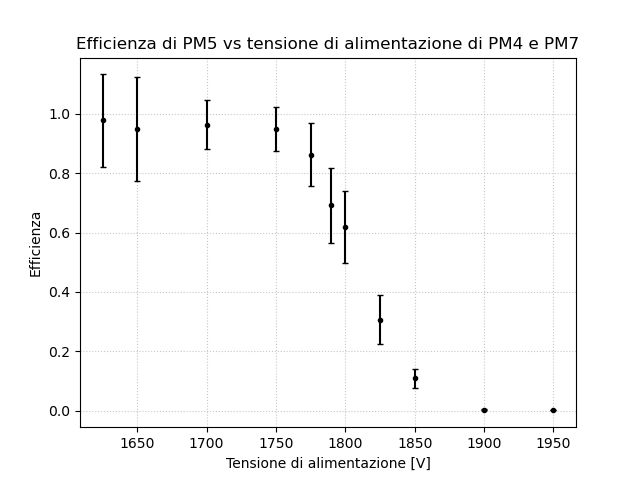
\includegraphics[scale=0.7]{Grafici/epsilon_vs_alimentazione_altri.png}
\caption{Efficienza $\epsilon_2$ al variare della tensione di alimentazione degli altri due fotomoltiplicatori PM4 e PM7} \label{facc}
\end{center}
\end{figure}

\newpage 
\subsubsection{Stima del numero di coincidenze accidentali}
\begin{table}[H]
\centering
\begin{tabular}{|c|c|c|c|c|c|c|}
\hline
PM & Alimentazione & Singola [cps] & $1 \& 2$  [cps] & $1 \& 2$ accidentali [cps]&  $1\&2\& 3$ [cps]& $\epsilon_3$\\ 
\hline 
PM7 & & $4.7 \pm 2.2$ & & & & \\ 
PM5 & 1625 & $119.6 \pm 10.9$& $0.9 \pm 0.9$  & $0.001$ & $0.9 \pm 0.9$& $0.98 \pm 1.04$ \\ 
PM4 & & $21.1 \pm 4.6$ & & & & \\ 
\hline 
PM7 & & $6.6 \pm 2.6$ & & & & \\ 
PM5 & 1650 & $124.9 \pm 11.2$& $1.6 \pm 1.3$  & $0.003$ & $1.5 \pm 1.2$& $0.95 \pm 0.78$ \\ 
PM4 & & $51.2 \pm 7.2$ & & & & \\ 
\hline 
PM7 & & $23.2 \pm 4.8$ & & & & \\ 
PM5 & 1700 & $123.8 \pm 11.1$& $5.0 \pm 2.2$  & $0.036$ & $4.8 \pm 2.2$& $0.96 \pm 0.44$ \\ 
PM4 & & $163.2 \pm 12.8$ & & & & \\ 
\hline 
PM7 & & $117.7 \pm 10.8$ & & & & \\ 
PM5 & 1750 & $124.7 \pm 11.2$& $8.8 \pm 3.0$  & $0.891$ & $8.4 \pm 2.9$& $0.95 \pm 0.33$ \\ 
PM4 & & $788.5 \pm 28.1$ & & & & \\ 
\hline 
PM7 & & $280.4 \pm 16.7$ & & & & \\ 
PM5 & 1775 & $118.3 \pm 10.9$& $10.5 \pm 3.2$  & $29$ & $9.1 \pm 3.0$& $0.86 \pm 0.29$ \\ 
PM4 & & $10758.8 \pm 103.7$ & & & & \\ 
\hline 
PM7 & & $335.6 \pm 18.3$ & & & & \\ 
PM5 & 1790 & $117.0 \pm 10.8$& $13.2 \pm 3.6$  & $114$ & $9.1 \pm 3.0$& $0.69 \pm 0.23$ \\ 
PM4 & & $35392.3 \pm 188.1$ & & & & \\ 
\hline 
PM7 & & $338.6 \pm 18.4$ & & & & \\ 
PM5 & 1800 & $127.7 \pm 11.3$& $15.8 \pm 4.0$  & $208$ & $9.8 \pm 3.1$& $0.62 \pm 0.20$ \\ 
PM4 & & $64017.0 \pm 253.0$ & & & & \\ 
\hline 
PM7 & & $568.2 \pm 23.8$ & & & & \\ 
PM5 & 1825 & $118.2 \pm 10.9$& $31.2 \pm 5.6$  & $732$ & $9.5 \pm 3.1$& $0.31 \pm 0.10$ \\ 
PM4 & & $134161.8 \pm 366.3$ & & & & \\ 
\hline 
PM7 & & $1602.2 \pm 40.0$ & & & & \\ 
PM5 & 1850 & $120.0 \pm 11.0$& $93.9 \pm 9.7$  & $2963$ & $10.2 \pm 3.2$& $0.11 \pm 0.03$ \\ 
PM4 & & $192670.5 \pm 438.9$ & & & & \\ 
\hline 
PM7 & & $56058.4 \pm 236.8$ & & & & \\ 
PM5 & 1900 & $117.8 \pm 10.9$& $3577.3 \pm 59.8$  & $130673$ & $10.1 \pm 3.2$&  $0.0028 \pm 0.0009$ \\ 
PM4 & & $242814.5 \pm 492.8$ & & & & \\ 
\hline 
PM7 & & $240242.2 \pm 490.1$ & & & & \\ 
PM5 & 1950 & $119.3 \pm 10.9$& $16377.5 \pm 128.0$  & $609510$ & $11.2 \pm 3.3$& $0.0007 \pm 0.0002$ \\ 
PM4 & & $264277.6 \pm 514.1$ & & & & \\ 
\hline
\end{tabular}
\caption{Conteggi per la stima di $\epsilon_2$}\label{tabacc}
\end{table}

Ho riportato il tabella \ref{tabacc}, oltre alle solite misure dei conteggi, anche una stima grossolana di coincidenze accidentali $1\&3$, tuttavia questi valori non hanno molto significato perché a partire dai 1775 V superano il numero totale di coincidenze doppie. 
\\
\\
Una possibile spiegazione può essere la seguente: il terzo fotomoltiplicatore (e poi anche il primo a tensioni più alte) per tensioni oltre i 1775 V produce un segnale molto rumoroso, che fa scattare l'unità di discriminazione anche in assenza di un segnale vero e proprio, perché la soglia di -40 mV diventa troppo bassa, come visto in figura \ref{fnoise}. 
\\
Osservando i conteggi in singola di PM4, si può anche ipotizzare che il suo segnale ad alimentazioni alte sia più rumoroso rispetto a quello di PM5, perché si hanno a 1900 V dei conteggi di 242814 per PM4 e di circa 1800 per PM5, ma non ho verificato direttamente all'oscilloscopio la forma del segnale.
\\
Inoltre, è anche possibile che ci siano state alcune riflessioni nei cavi coassiali che hanno aumentato i conteggi in singola di PM4 e PM7 e quindi falsano la stima dei conteggi accidentali.

\newpage
\section{Osservazione delle riflessioni nei cavi coassiali}
\end{document}



